%%% In this section, you will describe all of the various artifacts that you will generate and maintain during the project life cycle. Describe the purpose of each item below, how the content will be generated, where it will be stored, how often it will be updated, etc. Replace the default text for each section with your own description. Reword this paragraph as appropriate.

\subsection{Major Documentation Deliverables}
\subsubsection{Project Charter}
This document will only be updated when or if there are any changes in our vision, mission, success criteria, system overview, roles, budget, equipment, facilities, constraints, or risks. We plan on delivering our initial version on Tuesday October 1, 2019. The final version will be delivered the last week of class.
\subsubsection{System Requirements Specification}
The system requirements document will be started once we figure out all of our system requirements and if anything changes we will update the document accordingly.  The initial version will be delivered on October 22, 2019 and the final version will be submitted the last week of class.

\subsubsection{Architectural Design Specification}
The Architectural design specification document initial version will be delivered November 12, 2019 and the final version will be submitted the last week of class. The document will be updated as needed, meaning if there are any changes in the architectural design this includes the finest details.

\subsubsection{Detailed Design Specification}
The Detailed Design specification document initial version will be delivered on December 2, 2019 and this will be the final version. We assume the document will not need any updating we plan on having all aspects of the project in order.

\subsection{Recurring Sprint Items}
The following items will be documented and maintained during each individual sprint. As above, remove this paragraph from your draft, but leave the heading.

\subsubsection{Product Backlog}
Items will be added to the product backlog as we work through the previous requirements and then get to the new requirements. All SRS items will go through thorough analysis before being added to the product backlog, to gain a full understanding of all customer needs .Item prioritization will be done by the team lead and will be prioritized by which items needs immediate attention. Product backlog will be shared and updated through Google Drive.

\subsubsection{Sprint Planning}
How will each sprint plan be planned? How many sprints will there be (you need to look at the schedules for this course and previous Senior Design II courses during the appropriate semesters to figure this out).

\subsubsection{Sprint Goal}
The team lead ultimately decides the sprint goal, but sprint goals are suggested by the entire team including the customer. Sprint goals will go through thorough analysis before being added. The customer will be either on call or in person when going over the sprint goals.

\subsubsection{Sprint Backlog}
Team lead will decide which product backlog items make their way into the sprint backlog, after informing the team and getting everyone's perspective on the task. The document will be maintained on Google Sheets. 

\subsubsection{Task Breakdown}
Tasks will be assigned by team members volunteering to claim a task. In order to document the time spent on a task will be through a time in time out portion on excel. Team members will enter the time they started a task and stop a task each day, then we will calculate the hours spent on the task. This will be in the scrum excel file.

\subsubsection{Sprint Burn Down Charts}
Team Lead is responsible for generating the burn down charts for each sprint. The charts will be on Google Sheets and shared with all team members, every member is expected to fill out the total amount of effort expended. Effort will be calculated by the number of tasks completed each day. The format of the sprint burn down chart will be x = days, y = task remaining, estimated effort line, and actual effort line.

\begin{figure}[h!]
    \centering
    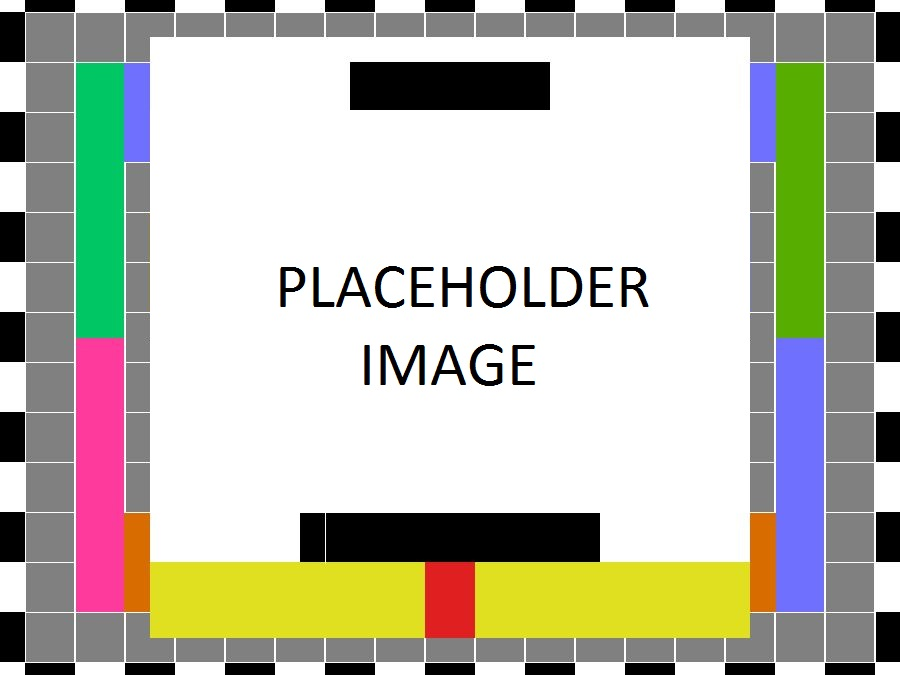
\includegraphics[width=0.5\textwidth]{images/test_image}
    \caption{Example sprint burn down chart}
\end{figure}

\subsubsection{Sprint Retrospective}
There will be a sprint retrospective discussion the day after the sprint presentation. We will examine the sprint if there are any recurring items we will go over why it is recurring and if there is anything that we missed or could do better next sprint. Notes on what to improve on the next sprint will be documented as individuals. 


\subsubsection{Individual Status Reports}
Individual status reports will be after every sprint on the task each person completed. There will be a report of what they learned including resources they used it will also include what we need to focus on as a team. The key items will be a suggestion for next sprint and resources they used.

\subsubsection{Engineering Notebooks}
The engineering notebook will have no minimum number of pages completed for each interval, we are unaware of how long an interval will be. The notebook will be updated when there is a meeting with the sponsor or when meeting with other teams. The engineering notebook will be used mainly for notes when in meeting. There is no need to hold members accountable due to there being no minimum. The witness will be the team lead or higher, meaning product owner or the sponsor. This way team lead is constantly in the loop with all incoming ideas. 

\subsection{Closeout Materials}
\subsubsection{System Prototype}
The final system prototype will be demonstrated to the sponsor in person with a Prototype Acceptance Test (PAT) this way we are able to clearly show our progress to the sponsor and find any faults. We plan on presenting the prototype before the actual demo day two weeks before. The final system prototype will include the automatic shutter system and both the android and iOS apps. During the presentation we will show the shutter opening and closing with the app from user input and then from a schedule.

\subsubsection{Project Poster}
The poster will a 28x40 inches elmer's tri fold corrugated project display board, it will include pictures of the individual hardware components, pictures of both apps, a summary of what our product is capable of, who the intended customers are, and our goals for the future . The poster will be delivered on demo day. 

\subsubsection{Web Page}
We plan on making a simple informative website that will be available to the public and be delivered on demo day. It will include information about our product and will have the vision and mission portion of this document, it will include links to the apps and information on how to use the product and to set up the product. It will be provided at closeout.


\subsubsection{Demo Video}
The demo video will be over setting the product up, it will be a how to video uploaded to YouTube, we will include b-reel footage with a voice over and text going over how to install the product and setting up the Bluetooth communication through the app. The video will be approximately 20 minutes or less .

\subsubsection{Source Code}
We plan on having a Creative Common Software License this is to protect against hacking, also we can say what end users can and can not do. Source code will be maintained on a private GitHub repository, the customer will not be given the source code to prevent hacking the less people who know the code the better. The license terms will be in each source file and we still have to decide whether or not to make our project public.

\subsubsection{Source Code Documentation}
We plan on using Doxygen to generate documentation and the final documentation will be provided as a PDF available on the website.

\subsubsection{Hardware Schematics}
Will you be creating printed circuit boards (PCBs) or wiring components together? If so, list each applicable schematic and what sort of data it will contain (PCB layout, wiring diagram, etc.). If your project is purely software, omit this section.
Our portion of the project will be purely software

\subsubsection{Installation Scripts}
Customers will have to install the app on either IOS or Android and then follow the step by step process in setting up their smart shutter.

\subsubsection{User Manual}
The user manual will be available in the box with every product the manual will also be available on the website alongside a youtube video. The app will include step by step instructions on setting up the product. 
